\documentclass[12pt]{article}
\usepackage{geometry}    
\usepackage{moreverb}   
\usepackage{fancyhdr}
\geometry{letterpaper}
\usepackage{algorithmic}             
\usepackage{algorithm}
\usepackage{array}     
\usepackage{hyperref}
\usepackage{graphicx}
\usepackage{fullpage}	
\usepackage{amsmath, amssymb, amsthm}
\usepackage{mathabx}
\usepackage{float}
\usepackage{bm}	
\graphicspath{ {data/}  {data/results} }
\usepackage{url}


\begin{document}

\title{CS 283 Final Project \\ Poisson Image Editing}
\date{Fall 2014}
\author{George Wu}

\maketitle

%%%%%%%%%%%%%%%%%%%%%%%%%%%%%%%%%%%%%%%%%%%%%%%%%%%%%
\section{Introduction}
What if you could seamlessly blend parts of images to make it seem as if those parts actually transpired in the same setting? As photography has shifted to the digital world, photo editing has become more accessible to the average consumer, with software such as Adobe Photoshop \cite{photoshop} and Lightroom \cite{lightroom} allowing such capabilities. Traditional methods involve directly copying and pasting portions of a source image's contents onto a background and blending the edges, but unless the source and background are already similar, these edges will still be visible. Adobe Photoshop \cite{photoshop} also has a Healing Brush, which has a similar result to poisson image editing \cite{poisson-paper}. We will explore ways to improve this process, borrowing heavily from the Poisson equation. Using a discrete version of the Poisson solver, we will be able to perform operations such as seamless cloning. 

%%%%%%%%%%%%%%%%%%%%%%%%%%%%%%%%%%%%%%%%%%%%%%%%%%%%%
\section{Methods}
\subsection{Discrete Poisson Solver}
To understand how the discrete poisson solver works, we will define some notation. Let $\Omega$ be the region to be solved for and its boundary $\partial \Omega$. Let $f$ be known values outside the interior of $\Omega$, and let $h$ be values to be solved for within $\Omega$. Let $v$ be a vector field over $\Omega$ that we will define based on the operation we are performing. For discrete images, we then want to perform the following minimization:
\begin{equation}
\min_{h \mid_\Omega} \sum_{\langle p,q\rangle \cap \Omega \neq \emptyset} (h_p-h_q- v_{pq})^2, \; h_p = f_p, \forall p \in \partial \Omega
\end{equation}
We can reformulate this problem as solving a system of linear equations 
\begin{equation}
\forall p \in \Omega, |N_p|h_p - \sum_{q\in N_p \cap \Omega} h_q = \sum_{q\in N_p\cap \partial \Omega} f_q + \sum_{q\in N_p} v_{pq}
\end{equation}
where $N_p$ is the set of horizontal and vertical neighbors of pixel $p$. In MATLAB, after forming the matrices that represent the system of equations, we can use the mldivide operator to determine the points.

\subsection{Seamless Cloning}
In the context of seamless cloning, $f$ represents our "destination image" or our "background image", which is the image we are pasting onto. We define $g$ to be the known values of the "source image" or the image we are pasting. $h$ is the values that we want to compute based on $f$ and $g$. To build the seamless cloner, we use the gradient of the source image as our value for $v$. With this we define
\begin{equation}
v_{pq} = g_p-g_q
\end{equation}
and we plug this value into equation $(2)$ and solve the system of equations. This allows us to retain the differences between pixels in the source image while keeping the boundaries consistent. This is implemented in \url{src/SeamlessCloning.m}. 

\subsection{Mixed Seamless Cloning}
With the seamless cloning method, within the region $\Omega$, we discarded all the information relating to the background or destination image. We can see that because for any pixel $p\in \Omega$, or $p$ is strictly within the region $\Omega$, equation $(2)$ becomes
\begin{equation}
\forall p \in \Omega, |N_p|h_p - \sum_{q\in N_p \cap \Omega} h_q = \sum_{q\in N_p} v_{pq}
\end{equation}
and we can see that this has no reliance on $f$, the background image. However, there are some scenarios where we would like to preserve the information in the background image. This is especially true when dealing with transparent objects, objects with holes, or cloning a region from the source image onto a region that overlaps with subjects in the background image. In this situation, we would like to keep the important parts of both images. In [Perez et al. 2003], the method described is to take the stronger of the two variations in the source and destination images. Therefore, we define
\begin{equation}
v_{pq} = 
\begin{cases}
f_p-f_q \;\; \text{if }|f_p - f_q|>|g_p-g_q|\\
g_p-g_q \;\; \text{otherwise} 
\end{cases}
\end{equation} 
and substitute this into equation $(2)$. 

\subsection{Texture Flattening}
In addition to performing cloning on two different images, we can use the poisson solver to edit portions of one image. Texture flattening is one of the many edits we can do, and [Perez et al. 2003] suggests using an edge detector. In this case, we will have
\begin{equation}
v_{pq} = 
\begin{cases}
f_p-f_q \;\; \textrm{there is an edge between $p$ and $q$}\\
0 \;\;\;\;\;\;\;\;\;\;\; \textrm{otherwise}
\end{cases}
\end{equation}
and we again substitute this into equation $(2)$ to solve. 

%%%%%%%%%%%%%%%%%%%%%%%%%%%%%%%%%%%%%%%%%%%%%%%%%%%%%
\section{Results} 
\subsection{Seamless Cloning}
\noindent\begin{figure}[H]
\centering
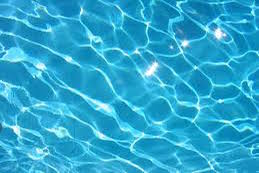
\includegraphics[width=0.49\textwidth,keepaspectratio]{data/SeamlessCloning/water/water_back.jpeg}
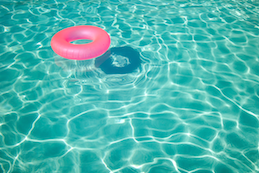
\includegraphics[width=0.49\textwidth,keepaspectratio]{data/SeamlessCloning/water/water_front.png}\\
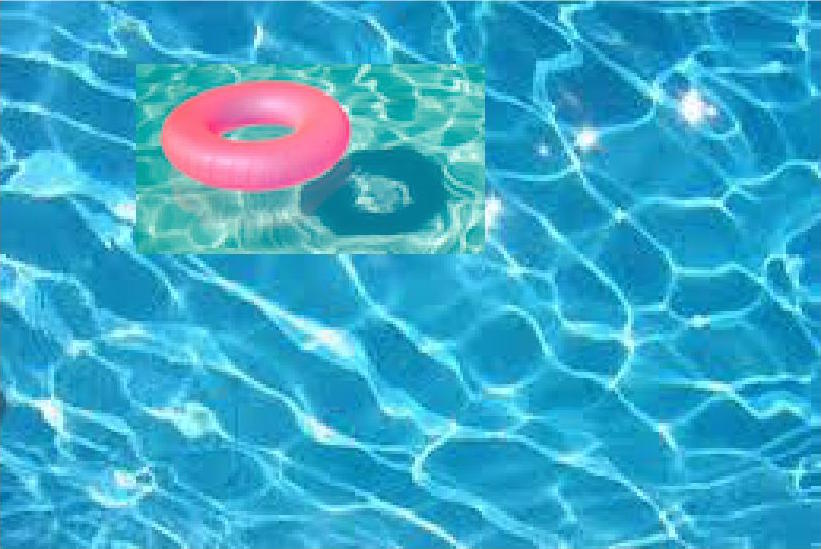
\includegraphics[width=0.49\textwidth,keepaspectratio]{data/SeamlessCloning/water/direct_pasting.jpg}
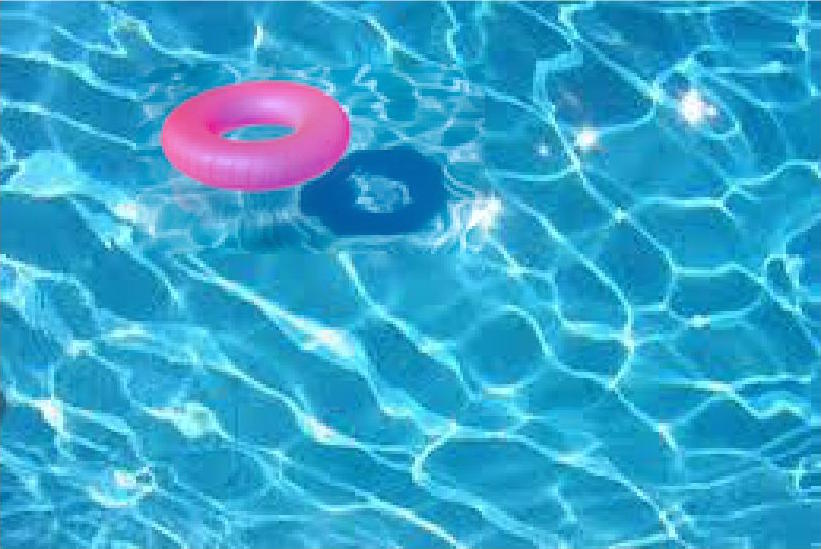
\includegraphics[width=0.49\textwidth,keepaspectratio]{data/SeamlessCloning/water/cloned.jpg}
\caption{Top left: Our destination or background image. Top right: Our source image. Bottom left: Image after directly pasting the source onto the destination. Bottom right: Image after applying Poisson Seamless Cloning. Seamless cloning achieves smoothness at the borders that regular image editing cannot match. At the same time, the color of the pool tube is more blue compared to the color in the original image.}
\label{water}
\end{figure}

We first tested our algorithm on two images of water, the source having an object clone over and the destination without any objects as shown in Figure \ref{water}. Because the textures of the two images are relatively similar, the resulting cloned image looks believable. One thing to notice is that along with the water surrounding the tube, the tube itself is now a deeper shade of blue, which could be an undesired effect.

\noindent\begin{figure}[H]
\centering
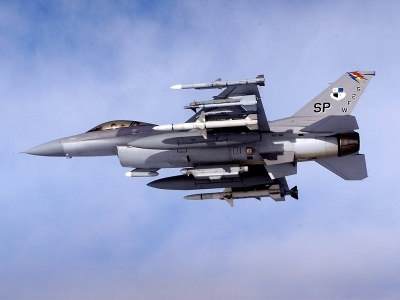
\includegraphics[width=0.25\textwidth,keepaspectratio]{data/SeamlessCloning/f16/F16Source.jpg}
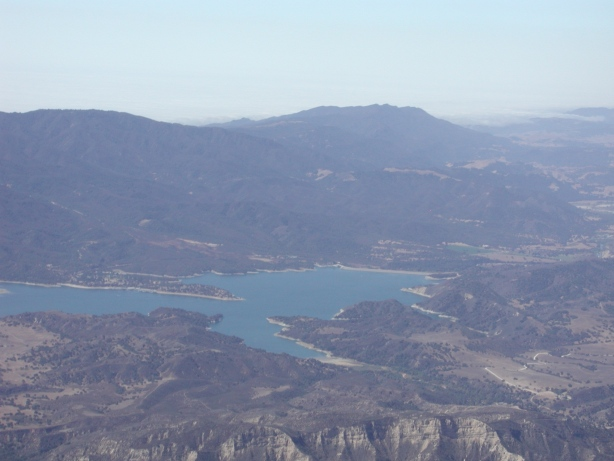
\includegraphics[width=0.25\textwidth,keepaspectratio]{data/SeamlessCloning/f16/F16Target.jpg}\\
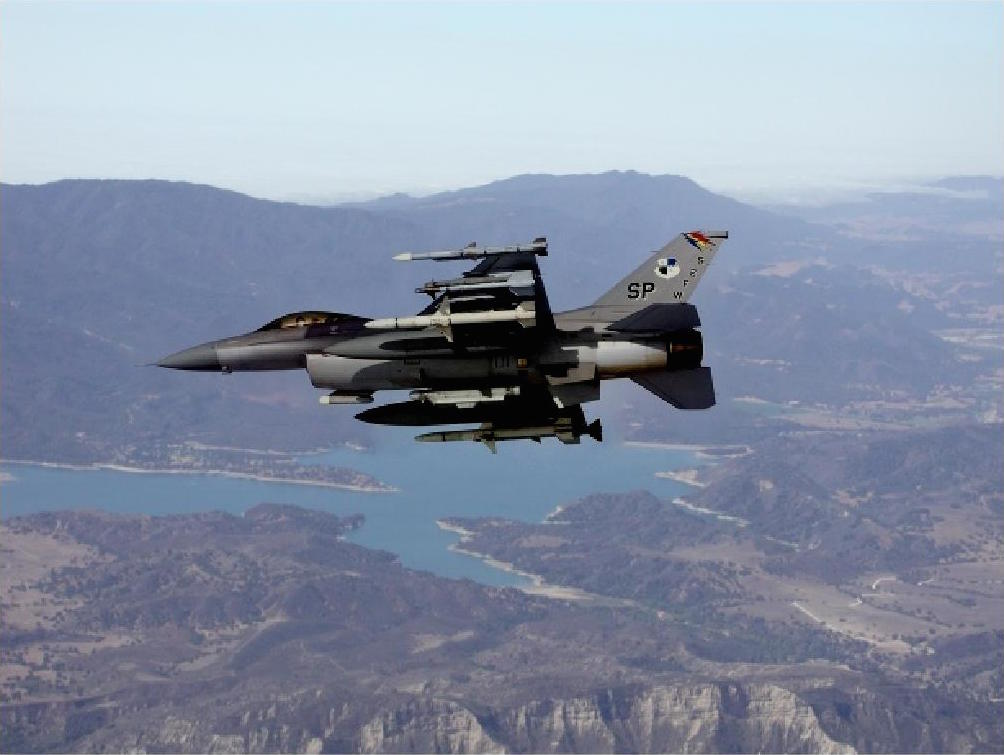
\includegraphics[width=0.35\textwidth,keepaspectratio]{data/SeamlessCloning/f16/cloned.jpg}
\caption{Top left: Our source image. Top right: Our destination or background image. Bottom: Image after applying Poisson Seamless Cloning. We notice that the seamless cloning adds a very slight halo around aircraft, probably due to the mask being larger than the actual aircraft.}
\label{f16}
\end{figure}

As shown in Figure \ref{f16}, the Poisson solver does quite well with these images. The color of the aircraft has changed to match the environment it is being pasted into.

In general, seamless cloning is good for directly masking over a background. If there is a big difference in texture between the source and the destination, then seamless cloning will result in noticeable changes in textures. In addition, if there large differences in color, then the color of the pasted region will change dramatically as well. Seamless cloning does not seem to do well with transparent objects or when adding an object in the source close to another object in the destination.

\subsection{Mixed Seamless Cloning}
Here we show an example where the regular seamless cloning leads to undesirable effects. 
\noindent\begin{figure}[H]
\centering
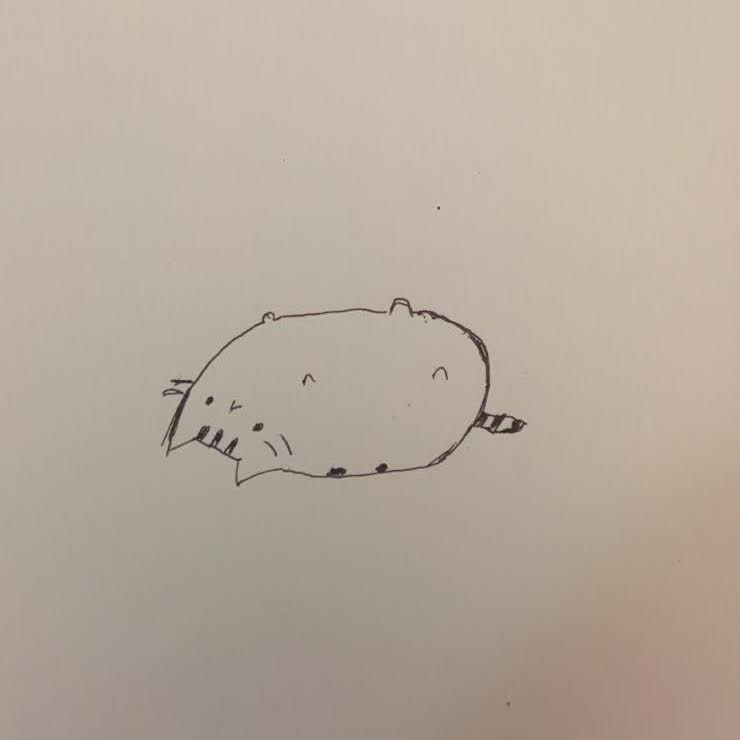
\includegraphics[width=0.24\textwidth,keepaspectratio]{data/MixedSeamlessCloning/mixed2/cat.jpg}
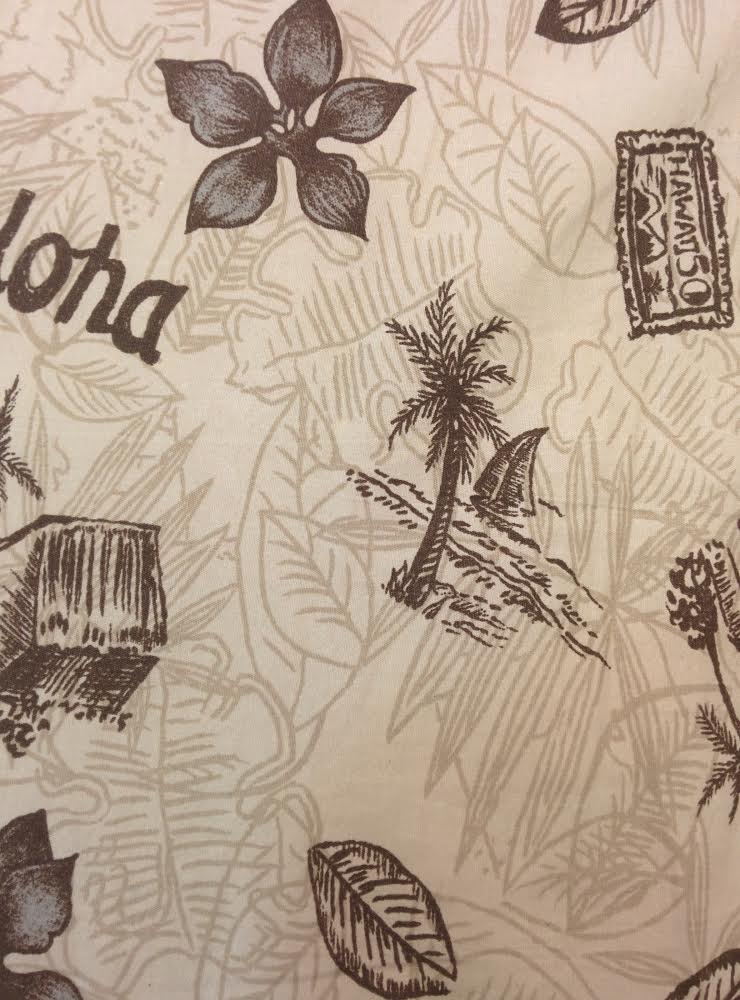
\includegraphics[width=0.24\textwidth,keepaspectratio]{data/MixedSeamlessCloning/mixed2/hawaii.jpg}
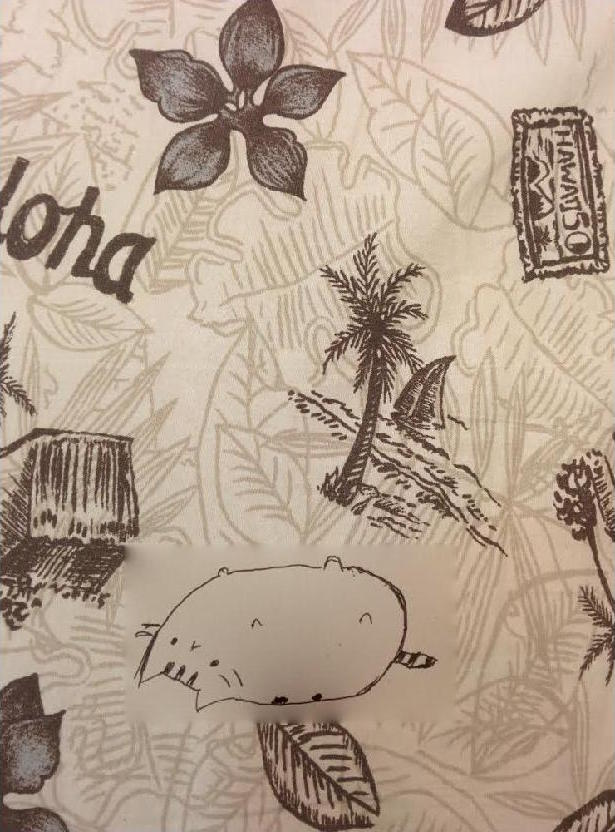
\includegraphics[width=0.24\textwidth,keepaspectratio]{data/MixedSeamlessCloning/mixed2/cloned.jpg}
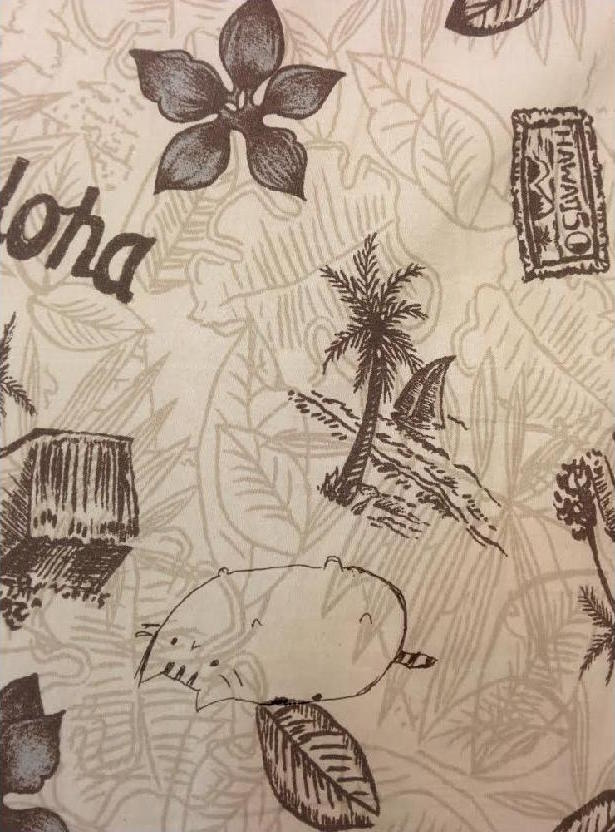
\includegraphics[width=0.24\textwidth,keepaspectratio]{data/MixedSeamlessCloning/mixed2/mixed_cloned.jpg}
\caption{Left: Our source image. Second from left: Our destination or background image. Second from right: Image after applying Poisson Seamless Cloning. Right: Image after applying Mixed Seamless Cloning. In this case, the source image is mostly hollow and produces an undesirable blur in the final image, which is taken out in the rightmost image.}
\label{cat-island}
\end{figure}
As we can see in Figure \ref{cat-island}, all the detail from the destination image in the pasted region is lost. By applying the mixed variant, we can achieve a better result. However, using the mixed variant is not always the best decision.

\noindent\begin{figure}[H]
\centering
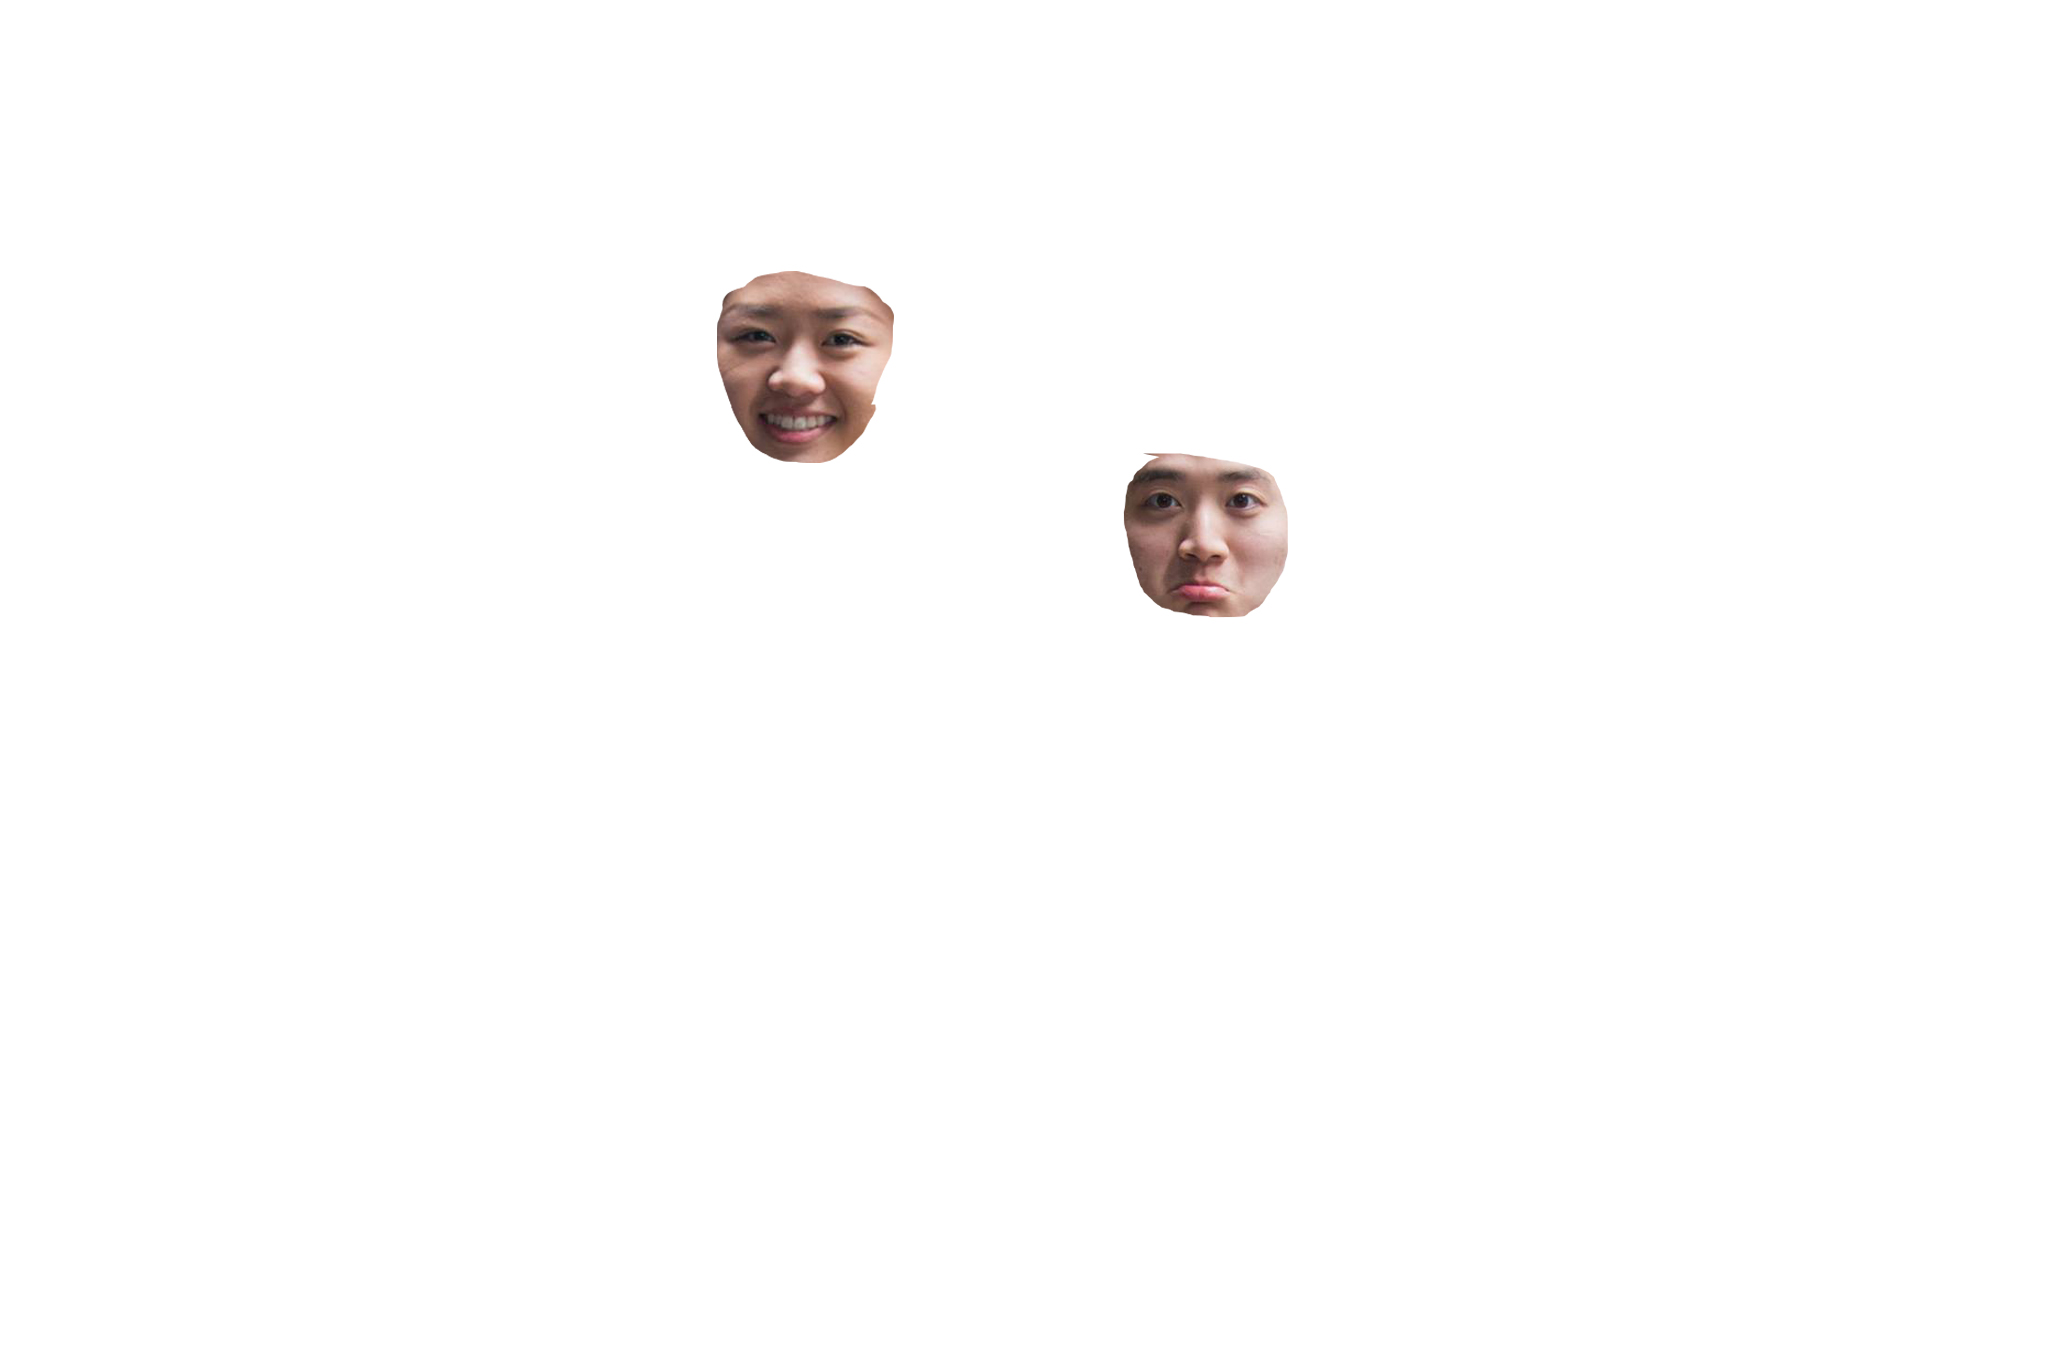
\includegraphics[width=0.24\textwidth,keepaspectratio]{data/SeamlessCloning/siblings/siblings_fore.jpg}
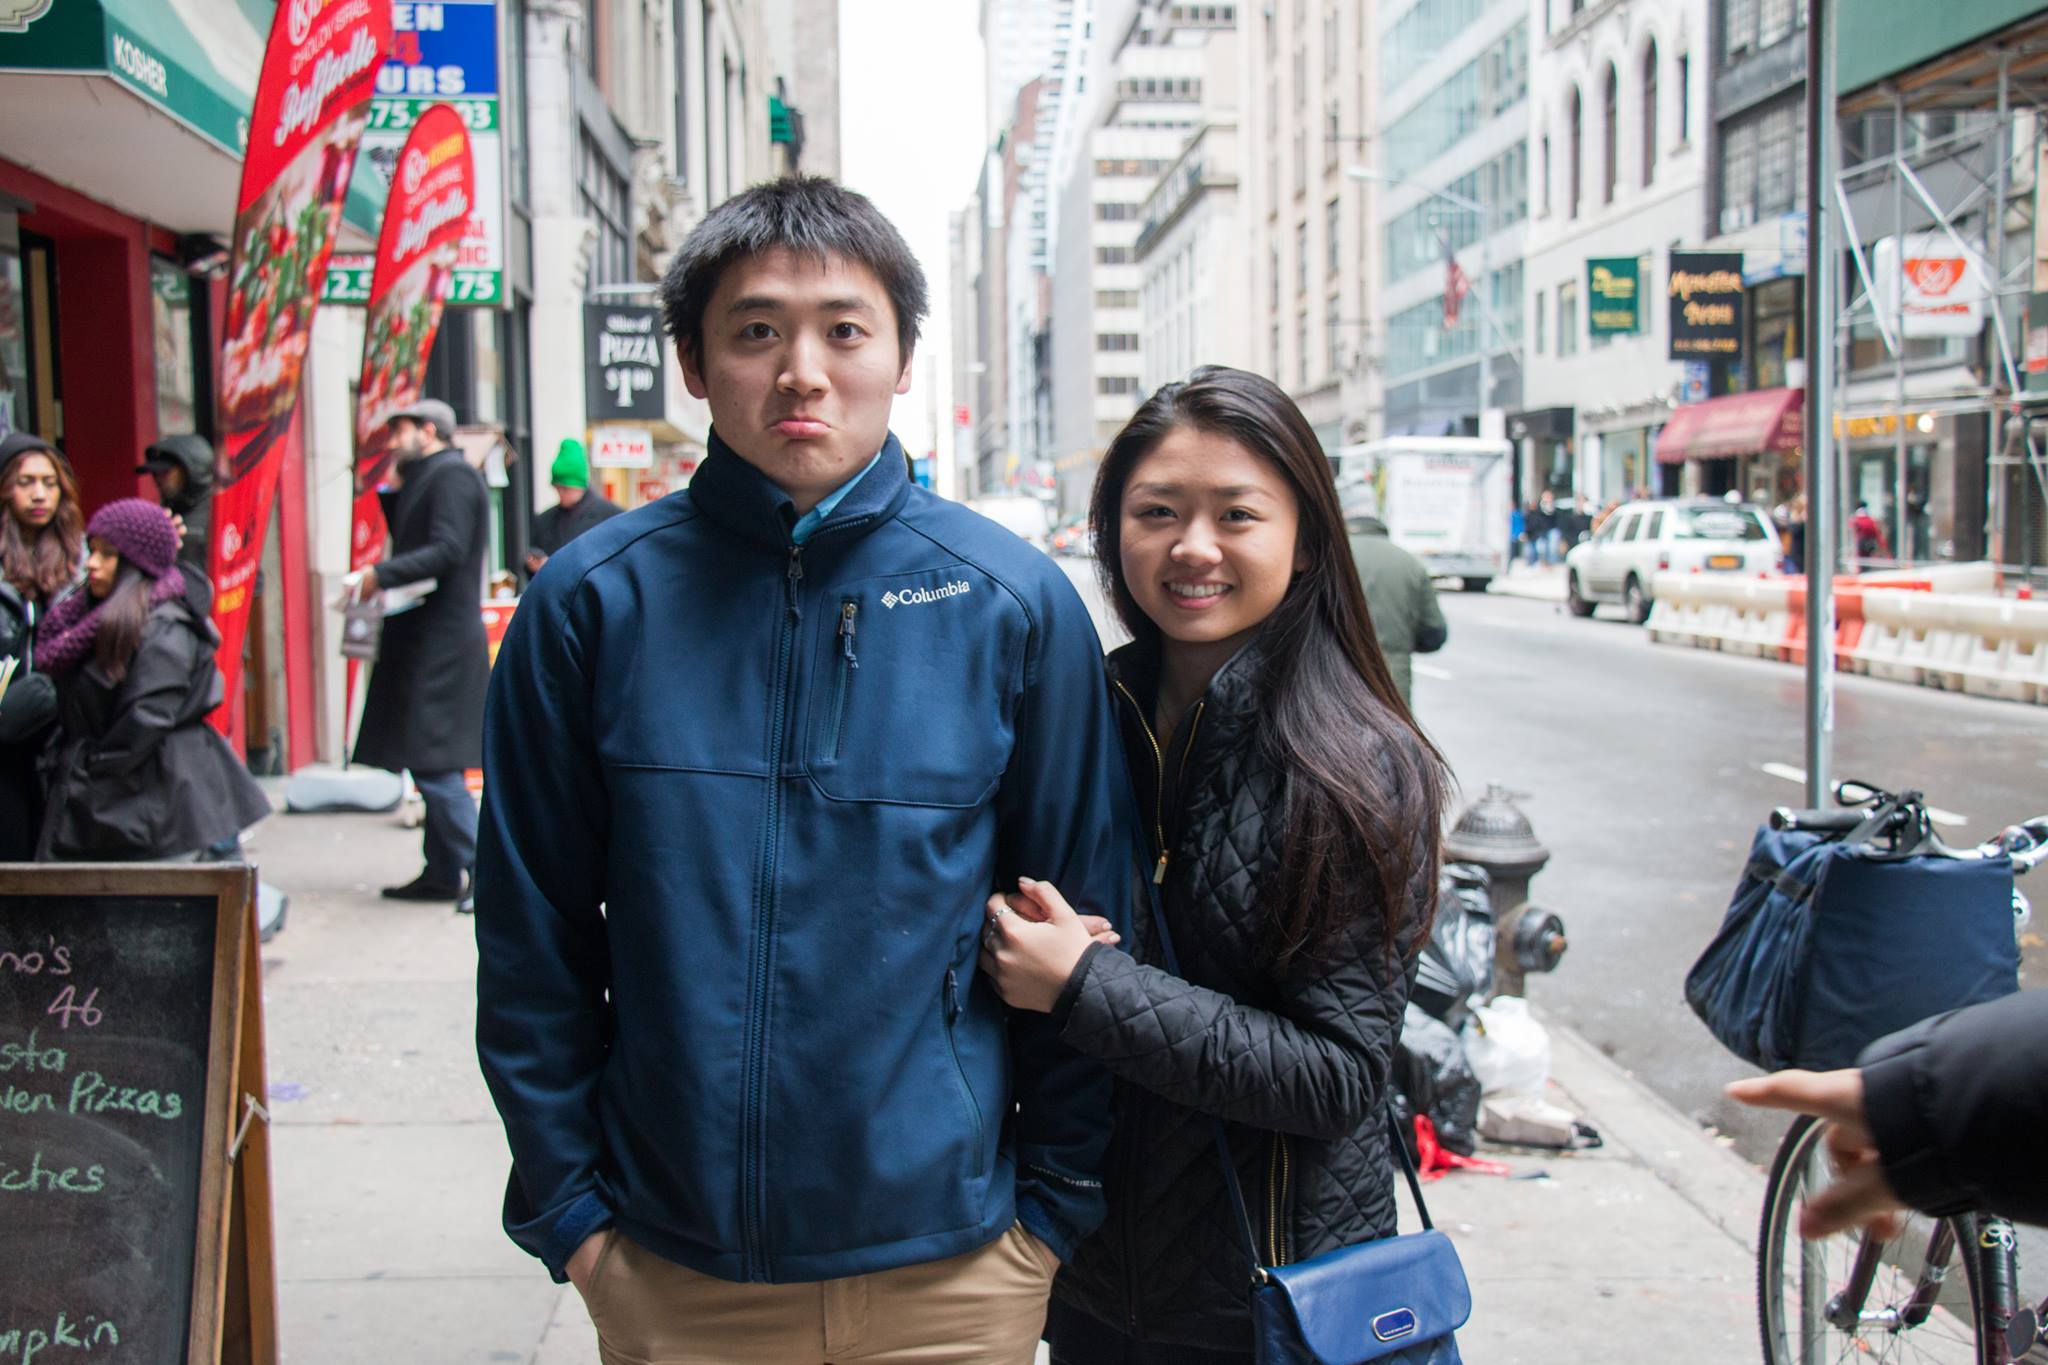
\includegraphics[width=0.24\textwidth,keepaspectratio]{data/SeamlessCloning/siblings/siblings.jpg}
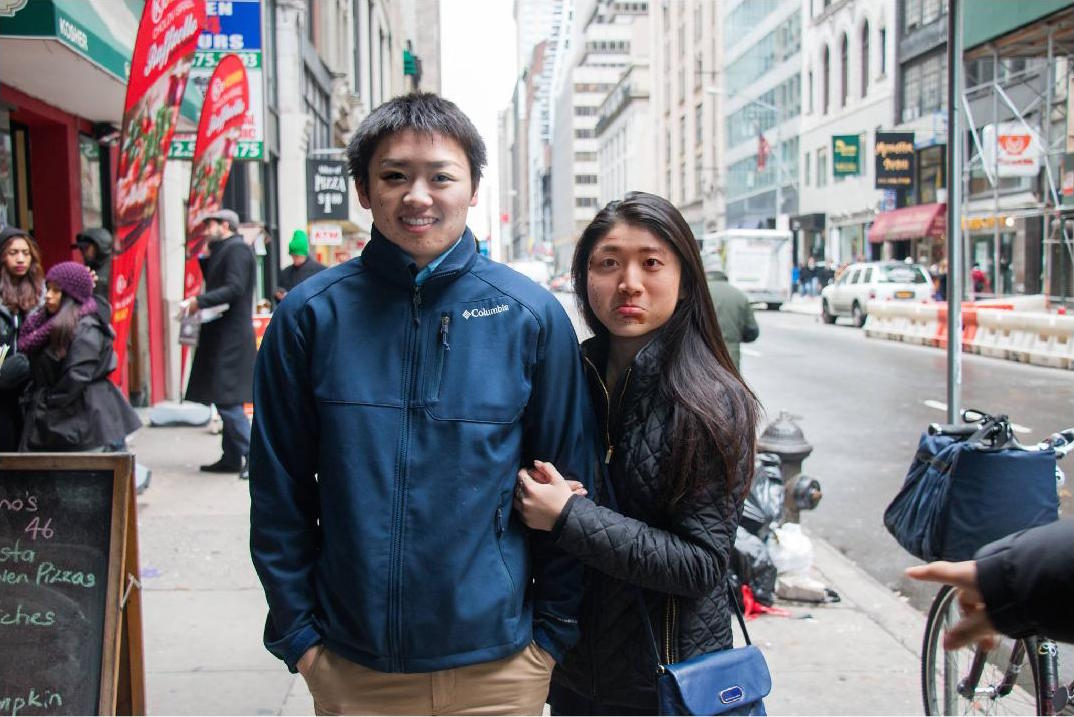
\includegraphics[width=0.24\textwidth,keepaspectratio]{data/SeamlessCloning/siblings/cloned.jpg}
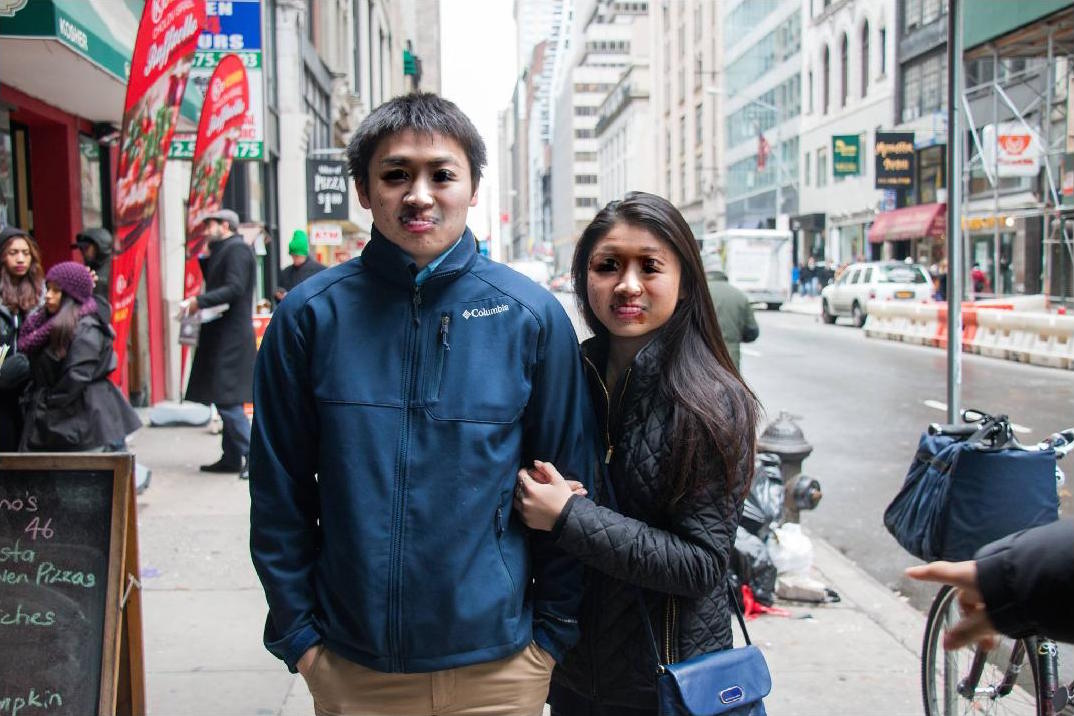
\includegraphics[width=0.24\textwidth,keepaspectratio]{data/SeamlessCloning/siblings/mixed_cloned.jpg}
\caption{Left: Our source image. Second from left: Our destination or background image. Second from right: Image after applying Poisson Seamless Cloning. Right: Image after applying mixed seamless cloning. Here we see that the original cloning is better than the mixed cloning, mostly because we do not want to preserve the details of the underlying faces.}
\label{siblings}
\end{figure}

In Figure \ref{siblings}, we would like to swap the faces of the two siblings in the picture. Inherently, this means that we do not want to preserve the original face detail, and so mixed seamless cloning is not the best method to approach this. It turns out that regular seamless cloning will do the job just fine.


\subsection{Texture Flattening}
\noindent\begin{figure}[H]
\centering
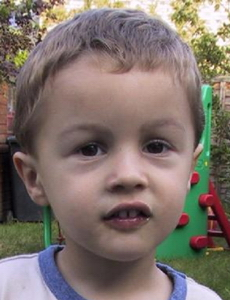
\includegraphics[width=0.4\textwidth,keepaspectratio]{data/TextureFlattening/child/child.jpg}
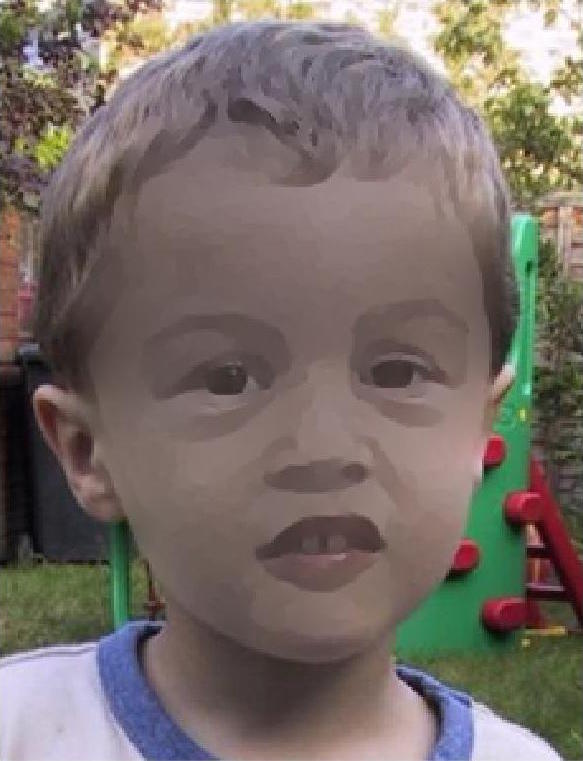
\includegraphics[width=0.4\textwidth,keepaspectratio]{data/TextureFlattening/child/texture_flatten.jpg}
\caption{Left: Original image. Right: Flattened image. Only the most significant edges are left visible, and the rest of the face has a flat structure.}
\label{child}
\end{figure}
Applying the flattening over the child's face, we see that we can still make out boundaries such as the eyes, nose, and lips of the child. 
\noindent\begin{figure}[H]
\centering
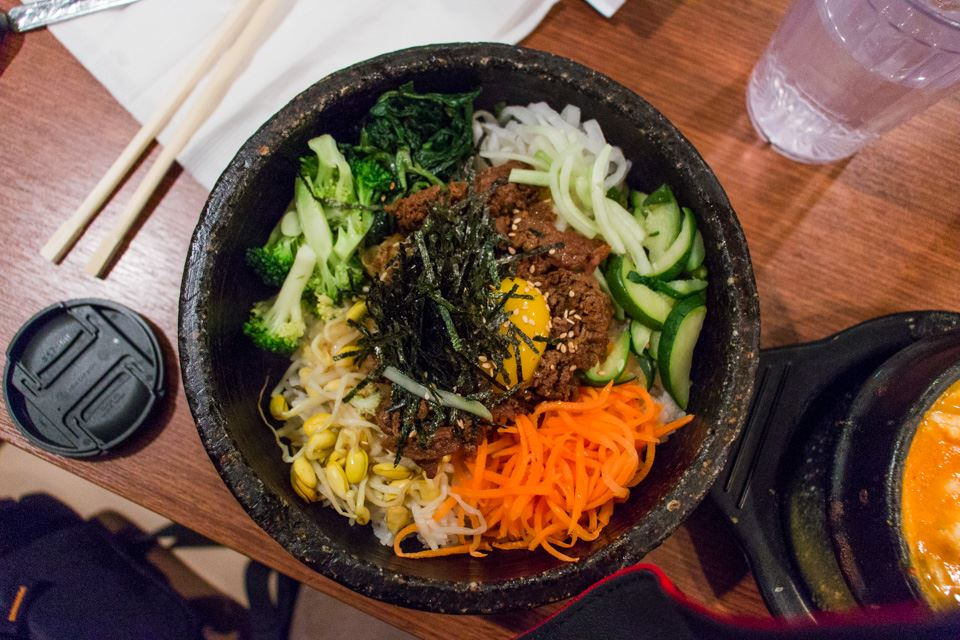
\includegraphics[width=0.4\textwidth,keepaspectratio]{data/TextureFlattening/food/food.jpg}
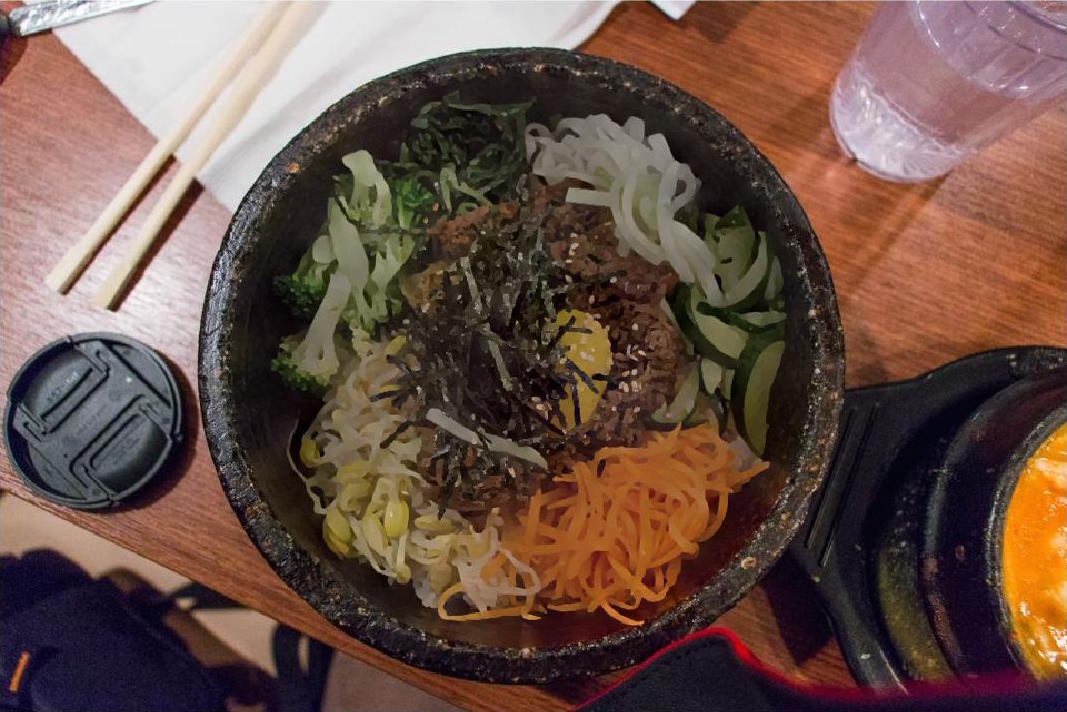
\includegraphics[width=0.4\textwidth,keepaspectratio]{data/TextureFlattening/food/texture_flatten.jpg}
\caption{Left: Original image. Right: Flattened image. The food in the center has a much flatter aspect, especially the broccoli and seaweed strips. The food also has lost much of its saturation.}
\label{child}
\end{figure}
%%%%%%%%%%%%%%%%%%%%%%%%%%%%%%%%%%%%%%%%%%%%%%%%%%%%%
\section{Conclusion}
Poisson image editing is a powerful tool that has a variety of uses. Perhaps its strongest features are that exact selection of an object is not required, and almost all of it is automated. In this paper, we explored many applications of poisson image editing such as seamless cloning and texture flattening. For the future, we would like to find ways to automatically correct for some side effects that these edits may bring about.

Seamless cloning changes the color of the entire region of the source image to match well with the destination image. While this is desirable in that it creates seamless boundaries, it also tends to change the subjects in the source images we are cloning. In some cases, such as in Figure \ref{f16}, it is not a noticeable problem, but if the source background and the destination background were significantly different, then we could see undesirable color changes in the subjects that we are cloning. One thing we would like to do is to detect what the subject in the source image is and try to maintain its color values so that the final image do not change.

Another interesting thing to automate would be to smartly detect whether regular seamless cloning or mixed seamless cloning would result in a better image and perform the better of the two. We hope that there are even more extensions that use the Poisson equation to edit photos.\\

\noindent{\bf Image Credits}
Child in Figure \ref{child} taken from [Perez et al. 2003].
%%%%%%%%%%%%%%%%%%%%%%%%%%%%%%%%%%%%%%%%%%%%%%%%%%%%%
\begin{thebibliography}{99}

\bibitem{lightroom}
Adobe Lightroom. Adobe, Inc. \textless\url{https://www.adobe.com/products/photoshop-lightroom.html?promoid=KLXLX}\textgreater

\bibitem{photoshop}
Adobe Photoshop. Adobe, Inc. \textless\url{http://www.adobe.com/products/photoshop.html}\textgreater.

\bibitem{matlab}
MATLAB documentation. \textless\url{http://www.mathworks.com/help/matlab/ref/mldivide.html}\textgreater.

\bibitem{poisson-paper}
P. Perez, M. Ganget, and A. Blake, "Poisson Image Editing." ACM Transactions on Graphics. 2003.
\end{thebibliography}


\end{document}